\part{Resultados}

\chapter[Resultados]{Resultados}\label{Capitulo5}

Este trabalho resultou em uma aplicação web 2.0 que ajuda na fase interna de licitação através de uma melhoria de comunicação.
Para atingirmos essas melhorias, nós mapeamos os problemas e criamos as soluções.
Soluções essas, que foram pensadas com vistas à centralizar para o usuário, informações atualizadas sobre processos licitatórios.

A fim de centralizar essas informações foi necessário obter dados sobre as licitações e também sobre itens, materiais, serviços e licitações, e vinculá-las ao nosso banco de dados
A obtenção desses dados é feita através de ação no sistema que recupera os dados na API de Compras Governamentais, forma pela qual o banco de dados pode se manter sempre atualizado com as licitações mais recentes.

Através dessa base de dados sempre atualizada, o usuário pode buscar na aplicação, material ou serviço pelo seu código ou descrição.

\begin{figure}[H]
	\centering
	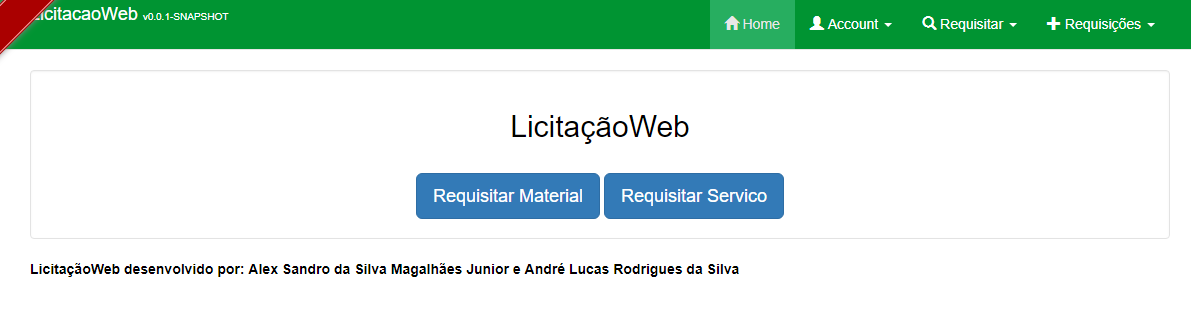
\includegraphics[width=0.95\textwidth]{figuras/prototipo001.png}
	\caption[PROT001: Tela home]{PROT001: Tela home.}
\end{figure}

\begin{figure}[H]
	\centering
	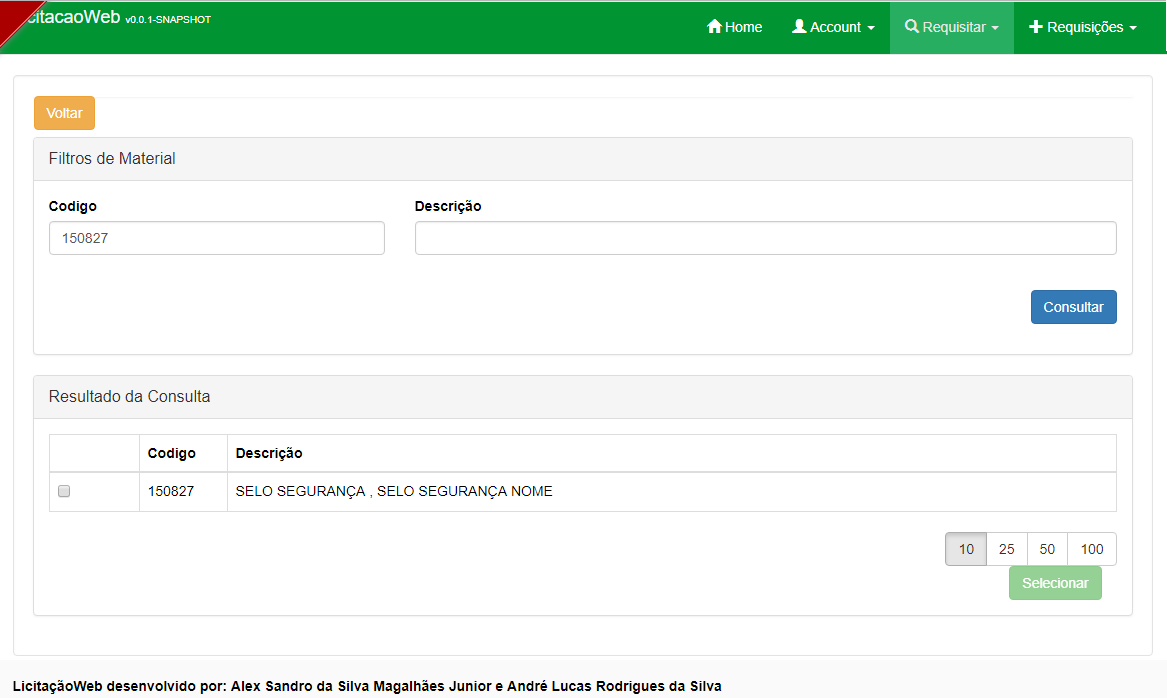
\includegraphics[width=0.95\textwidth]{figuras/prototipoA001.png}
	\caption[PROTA001: Solicitar Material]{PROTA001: Solicitar Material.}
\end{figure}

Isso permite que um câmpus interessado escolha uma licitação iniciada por outro câmpus para fazer sua adesão.

\begin{figure}[H]
	\centering
	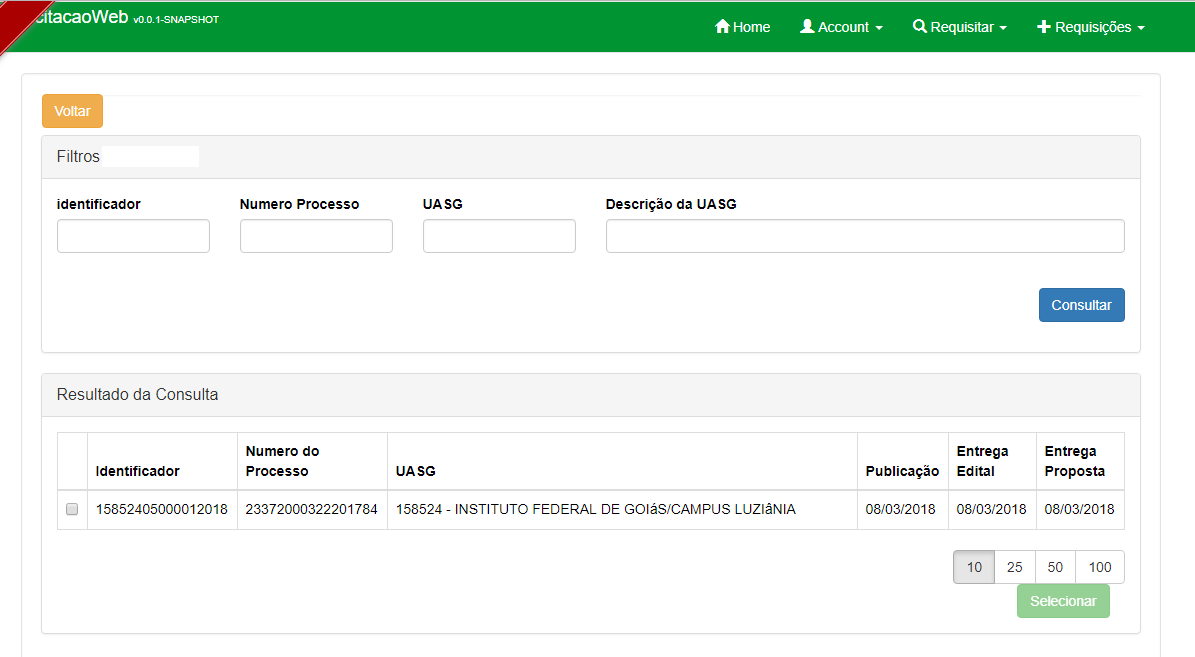
\includegraphics[width=0.95\textwidth]{figuras/prototipo002.png}
	\caption[PROT002: Licitações abertas]{PROT002: Licitações abertas.}
\end{figure}

indicando á quantidade de material ou serviço que gostaria de comprar junto.

\begin{figure}[H]
	\centering
	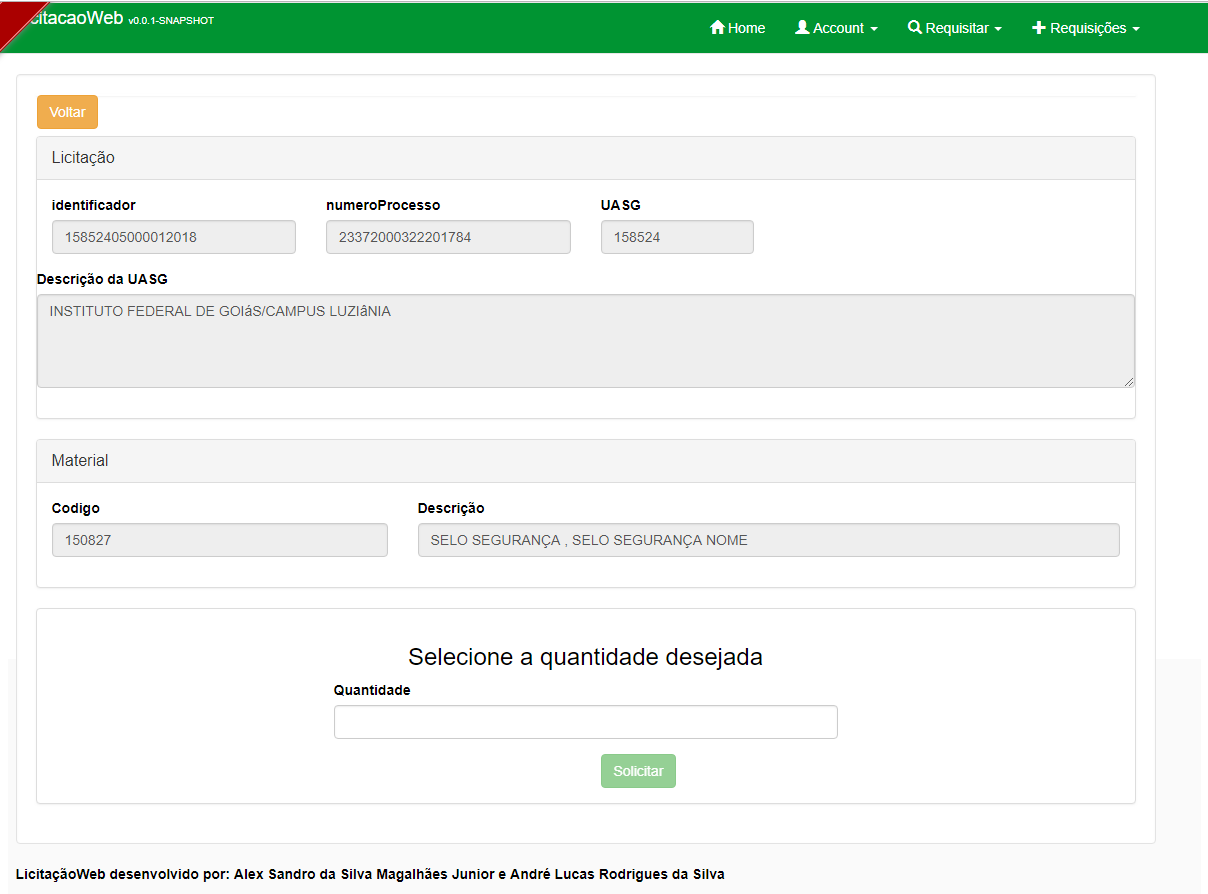
\includegraphics[width=0.95\textwidth]{figuras/prototipo003.png}
	\caption[PROT003: Descrição do item selecionado]{PROT003: Descrição do item selecionado.}
\end{figure}

Sempre que há uma solicitação, cada setor de compras dos \textit{campi} recebem uma requisição informando sobre um processo licitatório iniciado.

\begin{figure}[H]
	\centering
	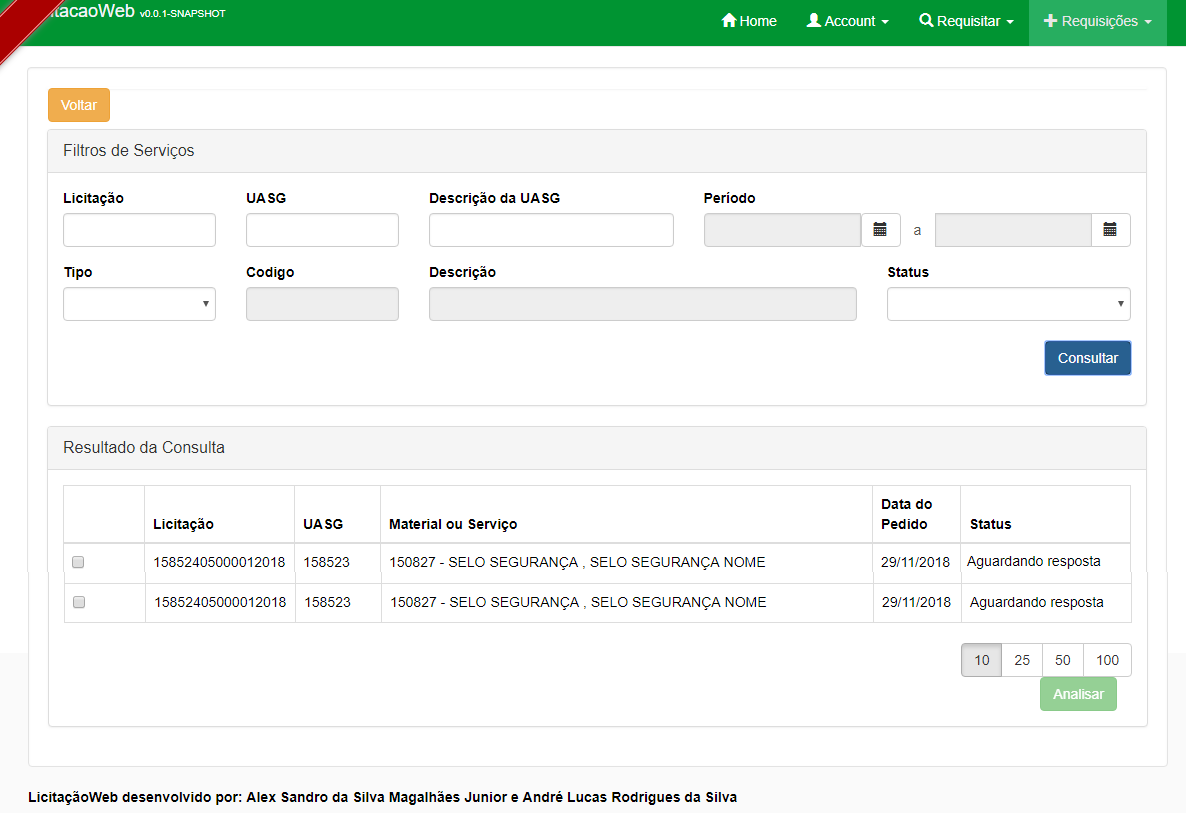
\includegraphics[width=0.95\textwidth]{figuras/prototipo006.png}
	\caption[PROT006: Lista de Requisições]{PROT006: Lista de Requisições.}
\end{figure}

O campûs destino analisa a requisição informando se aceita ou não.

\begin{figure}[H]
	\centering
	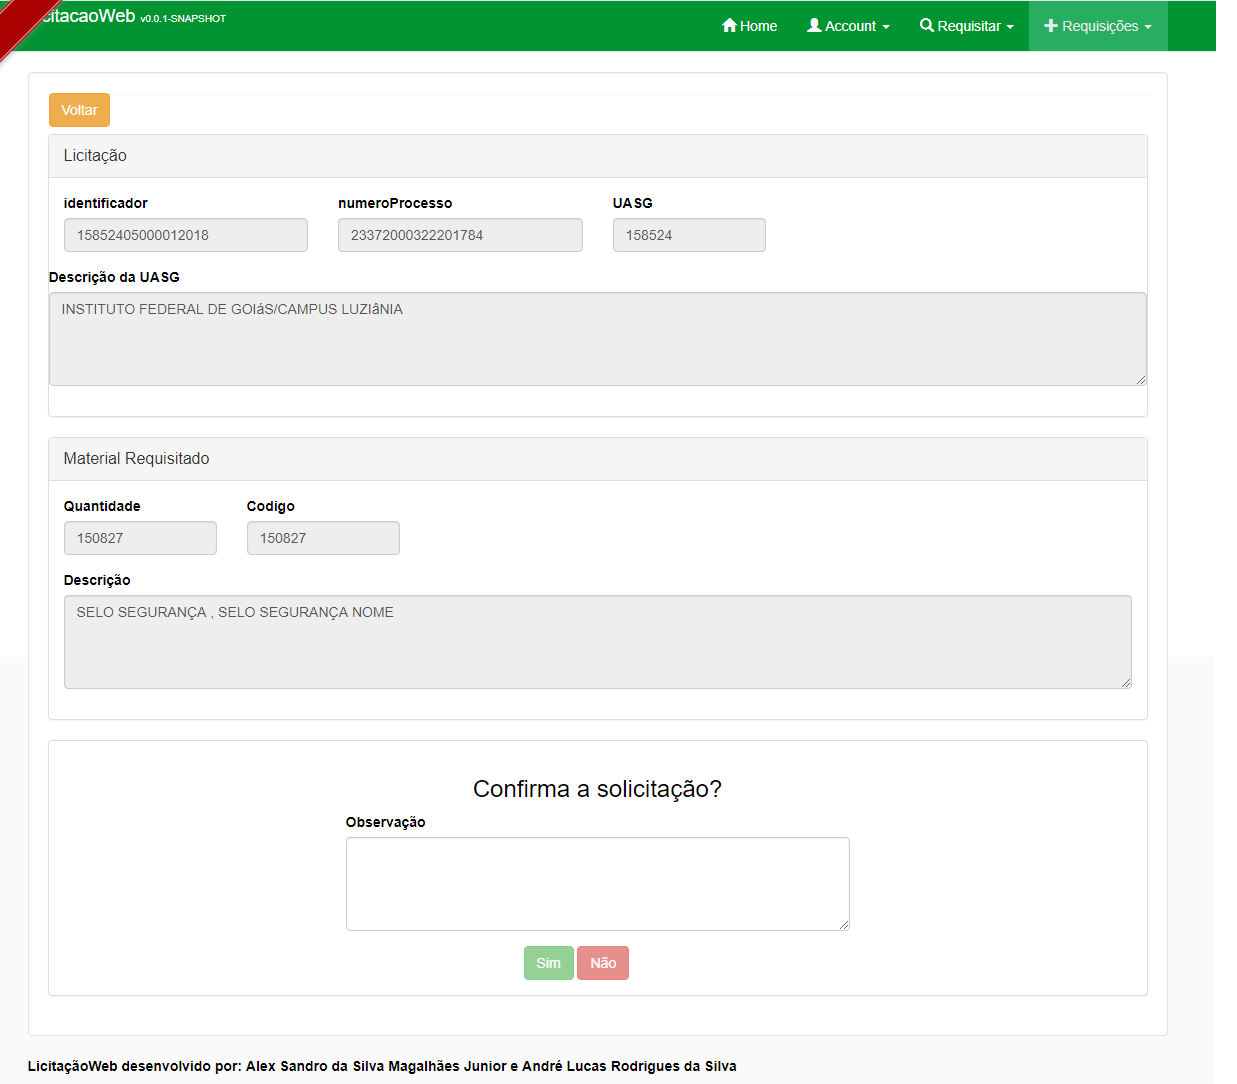
\includegraphics[width=0.95\textwidth]{figuras/prototipo007.png}
	\caption[PROT007: Analisar Requisições]{PROT007: Analisar Requisições.}
\end{figure}

Com a analise da requisição finalizada o campûs pedinte recebe á resposta da requisição.

\begin{figure}[H]
	\centering
	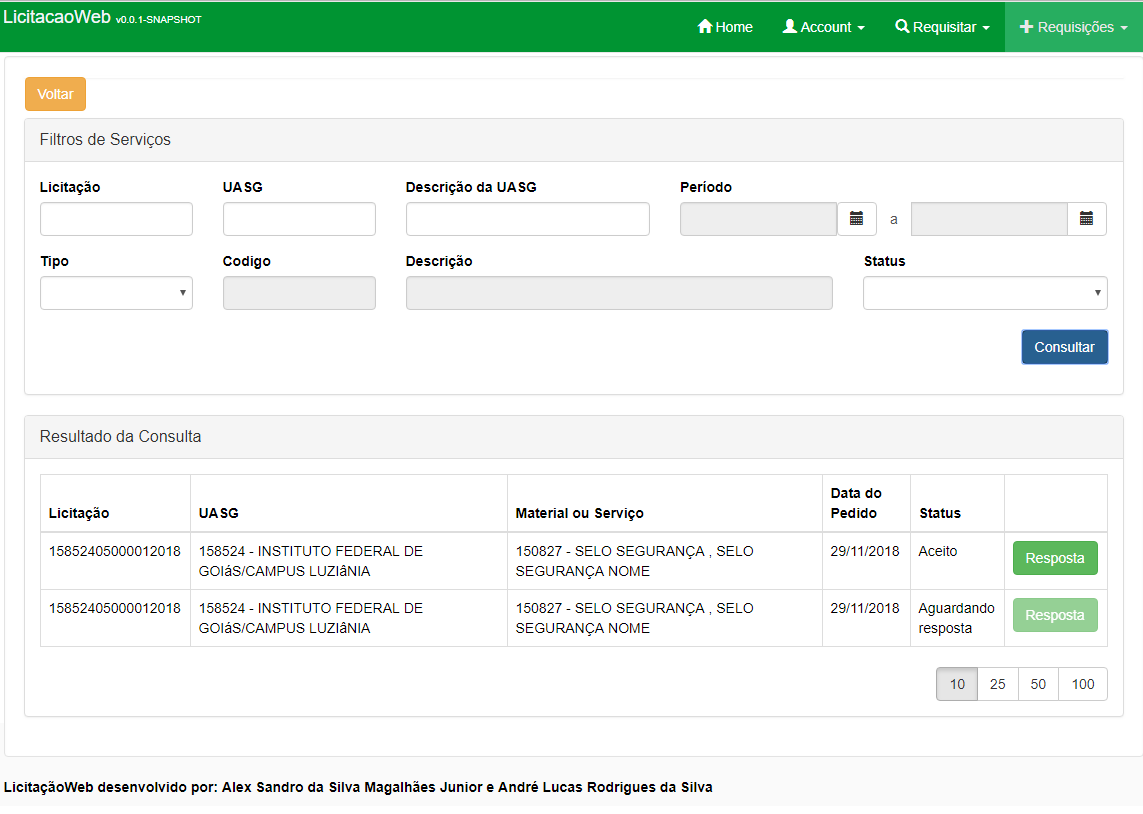
\includegraphics[width=0.95\textwidth]{figuras/prototipo009.png}
	\caption[PROT009: Lista de Requisições]{PROT009: Lista de Requisições.}
\end{figure}

\begin{figure}[H]
	\centering
	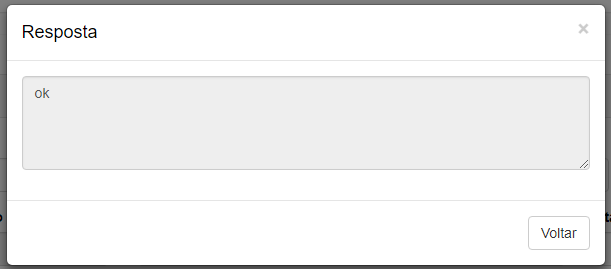
\includegraphics[width=0.95\textwidth]{figuras/prototipo010.png}
	\caption[PROT010: Resposta da Requisição]{PROT010: Resposta da Requisição.}
\end{figure}

O sistema desenvolvido agiliza um processo burocrático, dando celeridade na troca de informações sobre compras inter-\textit{campi}.


\section{Disponibilidade do Sistema}

Os sistema está disponível no GitHub no endereço:~\url{https://github.com/dragao1995/licitacaoweb} sob a Licença Apache 2.0.



